% ============================================================================
%  COMPILE WITH XeLaTeX  (twice, so the point total resolves)
%  Overleaf: Menu -> Compiler -> XeLaTeX
%  Requires: bnhandout.sty and fonts/Kalpurush.ttf in the project
% ============================================================================
\documentclass[11pt]{article}
\usepackage{bnhandout}          % add [nosol] for a student edition

\hauthor[https://sites.google.com/view/jugantordey/home]{Jugantor Dey}
\hseries{\textit{Mathematics for the Physics Olympiad}}

\begin{document}

\handouttitle{Chapter 15 : Differentiation}

\noindent
শুরু করার আগে ১৪ নম্বর অধ্যায় ভালোভাবে ঝালিয়ে নাও; বিশেষ করে limit-এর
সংজ্ঞা, limit-এর নিয়ম, এবং $\lim_{x \to 0} \dfrac{\sin x}{x} = 1$ ও
$\lim_{x \to 0} \dfrac{1-\cos x}{x^{2}} = \dfrac{1}{2}$ এই দুটি ফল। ৬ নম্বর
অধ্যায় থেকে ঢালের সংজ্ঞা আর ১৩ নম্বর অধ্যায় থেকে যোগ সূত্র লাগবে।
৮ নম্বর অধ্যায়ের binomial theorem একবার লাগবে, আর ৯ নম্বর অধ্যায়ের
নলাকার কৌটার সমস্যাটি পঞ্চম অনুচ্ছেদে ফিরে আসবে।

৬ নম্বর অধ্যায়ে সরলরেখার ঢাল বের করা শিখেছিলে, আর তখনই প্রশ্নটা উঠেছিল:
বাঁকা রেখার ঢাল বলতে কী বোঝায়? ১৪ নম্বর অধ্যায়ের শেষ অনুচ্ছেদে উত্তরটার
আকার দেখা গিয়েছিল: ছোট এলাকায় বক্ররেখাও প্রায় সরল, আর ``ছোট এলাকা'' কথাটার
নির্ভুল অর্থ দেয় limit।

সাতটি অনুচ্ছেদ, কিন্তু ভয়ের কিছু নেই; প্রথম চারটি একই জিনিসের চারটি স্তর।
প্রথমে ধারণা, তারপর সংজ্ঞা, তারপর সংজ্ঞা এড়িয়ে দ্রুত হিসাব করার নিয়ম, তারপর
সবচেয়ে শক্তিশালী নিয়মটি। শেষ তিনটি অনুচ্ছেদ ব্যবহার: চরম মান, একাধিক চলক, আর
ফাংশনকে polynomial দিয়ে বদলে ফেলা। এই অধ্যায়ে মোট \totalpoints\ পয়েন্ট
আছে।

\section{পরিবর্তনের হার}

একটি গাড়ি ২ ঘণ্টায় ১২০ কিলোমিটার গেল। গড় বেগ ঘণ্টায় ৬০ কিলোমিটার। কিন্তু
কোনো একটি নির্দিষ্ট মুহূর্তে তার বেগ কত ছিল? স্পিডোমিটার তো একটা সংখ্যা দেখায়;
সেটার মানে কী?

সমস্যাটা এই: বেগ মানে দূরত্ব ভাগ সময়, আর ``একটি মুহূর্তে'' সময়ের ব্যবধান
শূন্য, দূরত্বও শূন্য। $\dfrac{0}{0}$। ১৪ নম্বর অধ্যায় বলে দিয়েছে এই আকার
দেখে থেমে যেতে হয় না; limit নিতে হয়।

\begin{idea}[গড় ও তাৎক্ষণিক পরিবর্তনের হার]
$f$ ফাংশনের $x = a$ থেকে $x = a+h$ পর্যন্ত পরিবর্তনের গড় হার
\[
  \frac{f(a+h) - f(a)}{h} ,
\]
যা লেখচিত্রে $\bigl( a, f(a) \bigr)$ ও $\bigl( a+h, f(a+h) \bigr)$ বিন্দু দুটির
সংযোজক ছেদক রেখার (secant) ঢাল। $h \to 0$-এ এর limit-ই তাৎক্ষণিক পরিবর্তনের
হার, এবং সেটিই $( a, f(a) )$ বিন্দুতে স্পর্শকের (tangent) ঢাল।
\end{idea}

\begin{center}
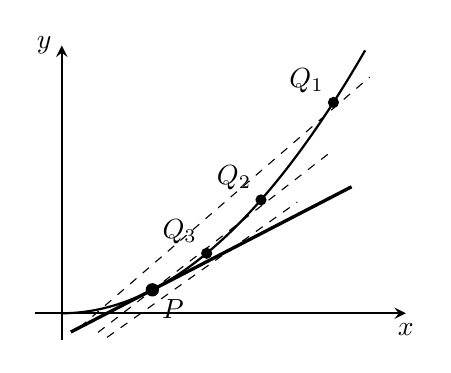
\begin{tikzpicture}[x=1.15cm,y=0.85cm,>=stealth]
  \draw[thick,->] (-0.3,0) -- (3.8,0) node[below] {$x$};
  \draw[thick,->] (0,-0.4) -- (0,4.0) node[left] {$y$};
  \draw[thick,domain=0:3.35,samples=80,variable=\x] plot ({\x},{0.35*\x*\x});
  \draw[dashed] (0.2,-0.21) -- (3.4,3.53);
  \draw[dashed] (0.4,-0.286) -- (3.0,2.44);
  \draw[dashed] (0.5,-0.36) -- (2.6,1.66);
  \draw[very thick] (0.1,-0.28) -- (3.2,1.89);
  \draw[fill] (1,0.35) circle (2.2pt) node[below right] {$P$};
  \draw[fill] (3,3.15) circle (1.8pt) node[above left] {$Q_{1}$};
  \draw[fill] (2.2,1.694) circle (1.8pt) node[above left] {$Q_{2}$};
  \draw[fill] (1.6,0.896) circle (1.8pt) node[above left] {$Q_{3}$};
\end{tikzpicture}
\end{center}

ছবিতে $Q$ বিন্দুটি $P$-এর দিকে এগোচ্ছে, আর ভাঙা রেখা তিনটি (secant) ক্রমে মোটা
রেখাটির (tangent) দিকে ঘুরে যাচ্ছে। খেয়াল করো, স্পর্শককে ``যে রেখা বক্ররেখাকে
একটি বিন্দুতে ছোঁয়'' বলে সংজ্ঞায়িত করা যায় না; বৃত্তের ক্ষেত্রে সেটি চলে,
কিন্তু সাধারণভাবে নয়। সঠিক সংজ্ঞা হলো: স্পর্শক হলো ছেদকদের limit।

\begin{example}
একটি বস্তুর $t$ সেকেন্ডে অতিক্রান্ত দূরত্ব $s(t) = 5t^{2}$ মিটার। $t = 2$
মুহূর্তে তার বেগ নির্ণয় করো।
\end{example}

\begin{solbox}
$t = 2$ থেকে $t = 2+h$ পর্যন্ত গড় বেগ:
\[
  \frac{s(2+h) - s(2)}{h}
  = \frac{5(2+h)^{2} - 20}{h}
  = \frac{5\left( 4 + 4h + h^{2} \right) - 20}{h}
  = \frac{20h + 5h^{2}}{h} .
\]
$h \neq 0$ বলে কাটাকাটি বৈধ, তাই রাশিটি $20 + 5h$। এখন
\[
  \lim_{h \to 0} (20 + 5h) = 20 .
\]
$t = 2$-এ বেগ ২০ মিটার প্রতি সেকেন্ড।

সংখ্যা দিয়ে যাচাই: $h = 0.1$-এ গড় বেগ $20.5$, $h = 0.01$-এ $20.05$,
$h = 0.001$-এ $20.005$। ঠিক $20$-এর দিকেই যাচ্ছে।
\end{solbox}

\prob{2} $s(t) = 4t^{2} + 3t$ (মিটার) হলে $t = 1$ থেকে $t = 1+h$ পর্যন্ত গড়
বেগ বের করো, এবং সেখান থেকে $t = 1$-এ তাৎক্ষণিক বেগ নির্ণয় করো।

\begin{sol}
\[
  s(1+h) = 4(1+h)^{2} + 3(1+h) = 4 + 8h + 4h^{2} + 3 + 3h = 7 + 11h + 4h^{2} ,
\]
আর $s(1) = 7$। সুতরাং গড় বেগ
\[
  \frac{11h + 4h^{2}}{h} = 11 + 4h \qquad (h \neq 0) .
\]
$h \to 0$-এ limit $11$, অর্থাৎ তাৎক্ষণিক বেগ ১১ মিটার প্রতি সেকেন্ড।
\end{sol}

\prob{2} সংজ্ঞা ব্যবহার করে $y = \dfrac{1}{x}$ বক্ররেখার $x = 2$ বিন্দুতে
স্পর্শকের ঢাল নির্ণয় করো।

\begin{sol}
\[
  \frac{f(2+h)-f(2)}{h}
  = \frac{\dfrac{1}{2+h} - \dfrac{1}{2}}{h}
  = \frac{\dfrac{2 - (2+h)}{2(2+h)}}{h}
  = \frac{-h}{2h(2+h)} = \frac{-1}{2(2+h)} .
\]
$h \to 0$-এ এটি $-\dfrac{1}{4}$। ঢাল ঋণাত্মক, যা মানানসই: $1/x$ ধনাত্মক
দিকে হ্রাসমান।
\end{sol}

\section{সংজ্ঞা থেকে ডেরিভেটিভ}

\begin{idea}[Derivative]
ফাংশন $f$-এর $x = a$ বিন্দুতে derivative
\[
  f'(a) = \lim_{h \to 0} \frac{f(a+h) - f(a)}{h} ,
\]
যদি এই limit-টির অস্তিত্ব থাকে। থাকলে $f$-কে বলা হয় $a$ বিন্দুতে
differentiable। প্রতিটি $x$-এ এভাবে পাওয়া মানগুলো নিয়ে যে নতুন ফাংশন তৈরি হয়,
তাকে বলে derivative function $f'$।
\end{idea}

লেখার কয়েকটি উপায় আছে, সবগুলোই একই জিনিস:
\[
  f'(x), \qquad \frac{df}{dx}, \qquad \frac{dy}{dx}, \qquad \dot{y} .
\]
শেষেরটি পদার্থবিজ্ঞানে ব্যবহৃত হয় এবং সবসময় সময়ের সাপেক্ষে derivative বোঝায়। একে ডট নোটেশন বলে।
একটি সতর্কতা: $\dfrac{dy}{dx}$ দেখতে ভগ্নাংশের মতো, কিন্তু এই মুহূর্তে সেটি
একটি অখণ্ড প্রতীক, ভগ্নাংশ নয়; $dy$ ও $dx$ আলাদা করে কী বোঝায় তা ১৬ নম্বর
অধ্যায়ের বিষয়।

\begin{example}
সংজ্ঞা থেকে $f(x) = \sqrt{x}$-এর derivative নির্ণয় করো ($x > 0$)।
\end{example}

\begin{solbox}
\[
  \frac{\sqrt{x+h} - \sqrt{x}}{h}
  = \frac{(x+h) - x}{h\left( \sqrt{x+h} + \sqrt{x} \right)}
  = \frac{1}{\sqrt{x+h} + \sqrt{x}} ,
\]
যেখানে অনুবন্ধী দিয়ে গুণ করা হয়েছে (১৪ নম্বর অধ্যায়ের দ্বিতীয় কৌশল)।
$h \to 0$-এ limit
\[
  f'(x) = \frac{1}{2\sqrt{x}} .
\]
$x = 9$-এ এটি $\dfrac{1}{6}$, যা ১৪ নম্বর অধ্যায়ের শেষ উদাহরণে সংখ্যা
দিয়ে পাওয়া গিয়েছিল।
\end{solbox}

\begin{idea}[Differentiable হলে continuous]
$f$ যদি $a$-তে differentiable হয়, তবে সে $a$-তে continuous।
\end{idea}

প্রমাণ এক লাইনের:
\[
  f(a+h) - f(a) = h \cdot \frac{f(a+h)-f(a)}{h}
  \;\longrightarrow\; 0 \cdot f'(a) = 0 ,
\]
অর্থাৎ $h \to 0$-এ $f(a+h) \to f(a)$, যা ঠিক continuity-র সংজ্ঞা।

উল্টোটা কিন্তু সত্য নয়, আর সেটাই এই অনুচ্ছেদের সবচেয়ে দরকারি বিষয়।

\begin{center}
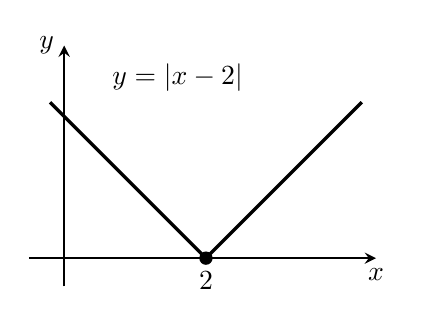
\begin{tikzpicture}[x=0.9cm,y=0.9cm,>=stealth]
  \draw[thick,->] (-0.5,0) -- (4.4,0) node[below] {$x$};
  \draw[thick,->] (0,-0.4) -- (0,3.0) node[left] {$y$};
  \draw[very thick] (-0.2,2.2) -- (2,0) -- (4.2,2.2);
  \draw[fill] (2,0) circle (2.2pt);
  \node[below] at (2,-0.05) {$2$};
  \node at (1.6,2.55) {$y=|x-2|$};
\end{tikzpicture}
\end{center}

$f(x) = |x-2|$ ফাংশনটি $x = 2$-এ continuous (কোনো লাফ নেই), কিন্তু
differentiable নয়। কারণ ডান দিক থেকে
\[
  \frac{f(2+h)-f(2)}{h} = \frac{|h|}{h} = 1 \quad (h > 0) ,
\]
আর বাম দিক থেকে ওই একই রাশি $-1$। দুই পাশের limit আলাদা, তাই limit নেই, তাই
derivative নেই। ছবিতে ব্যাপারটা স্পষ্ট: কোণার বিন্দুতে ``একটিমাত্র স্পর্শক''
বলে কিছু নেই।

\begin{remark}
পদার্থবিজ্ঞানে এই পার্থক্যটার মানে আছে। বেগ-সময় লেখচিত্রে কোণা মানে
তাৎক্ষণিক ত্বরণ অসংজ্ঞায়িত, অর্থাৎ ওই মুহূর্তে অসীম বল লাগত। বাস্তব ব্যবস্থায়
তা হয় না, তাই কোণাওয়ালা মডেল সবসময়ই একটি আসন্নীকরণ; খুব ছোট সময়ে ব্যাপারটা
আসলে মসৃণ।
\end{remark}

\prob{2} সংজ্ঞা থেকে $f(x) = x^{2} - 3x$-এর derivative নির্ণয় করো।

\begin{sol}
\[
  f(x+h) - f(x) = \left[ (x+h)^{2} - 3(x+h) \right] - \left[ x^{2}-3x \right]
  = 2xh + h^{2} - 3h .
\]
$h$ দিয়ে ভাগ করে $2x + h - 3$, আর $h \to 0$-এ limit
\[
  f'(x) = 2x - 3 .
\]
যাচাই: $x = 1.5$-এ $f' = 0$, আর parabola-টির শীর্ষবিন্দু সত্যিই $x = 1.5$-এ।
\end{sol}

\prob{3} সংজ্ঞা থেকে $f(x) = \sqrt{x+1}$-এর derivative নির্ণয় করো, এবং domain
নিয়ে কী সাবধানতা লাগে তা বলো।

\begin{sol}
\[
  \frac{\sqrt{x+1+h} - \sqrt{x+1}}{h}
  = \frac{(x+1+h) - (x+1)}{h\left( \sqrt{x+1+h} + \sqrt{x+1} \right)}
  = \frac{1}{\sqrt{x+1+h} + \sqrt{x+1}} ,
\]
তাই
\[
  f'(x) = \frac{1}{2\sqrt{x+1}} .
\]
Domain: $f$ নিজে সংজ্ঞায়িত $x \geq -1$-এ, কিন্তু $f'$ সংজ্ঞায়িত কেবল
$x > -1$-এ, কারণ $x = -1$-এ হর শূন্য হয়ে যায়। ওই প্রান্তবিন্দুতে স্পর্শক
উল্লম্ব, ঢাল অসীম। অর্থাৎ derivative-এর domain মূল ফাংশনের domain-এর চেয়ে
ছোট হতে পারে।
\end{sol}

\prob{3} $f(x) = |x-2|$ ফাংশনটি $x = 2$-এ continuous অথচ differentiable নয়,
সংজ্ঞা ব্যবহার করে দেখাও। এরপর $g(x) = (x-2)|x-2|$ ফাংশনটির জন্য একই প্রশ্নের
উত্তর দাও।

\begin{sol}
$f$-এর জন্য: $\lim_{x \to 2} |x-2| = 0 = f(2)$, তাই continuous। কিন্তু $\frac{f(2+h)-f(2)}{h} = \frac{|h|}{h}$
\[
  \lim_{h \to 0^{+}} \frac{|h|}{h} = 1, \qquad
  \lim_{h \to 0^{-}} \frac{|h|}{h} = -1 ,
\]
দুই পাশ আলাদা, তাই $f'(2)$-এর অস্তিত্ব নেই।

$g$-এর জন্য: $g(2) = 0$ এবং
\[
  \frac{g(2+h) - g(2)}{h} = \frac{h|h|}{h} = |h| .
\]
$h \to 0$-এ এটি $0$-তে যায়, দুই পাশ থেকেই। সুতরাং $g'(2) = 0$ এবং $g$
differentiable।

শিক্ষণীয়: $|x-2|$-এর কোণাটি $(x-2)$ দিয়ে গুণ করায় মসৃণ হয়ে গেছে। কোণা থাকা
না থাকা ফাংশনের গঠনের উপর নির্ভর করে, নিছক পরম মান চিহ্ন দেখে বলা যায় না।
\end{sol}

\section{নিয়মসমূহ}

সংজ্ঞা থেকে প্রতিবার limit নেওয়া অসম্ভব। ভাগ্য ভালো, derivative (যা এক ধরণের limit) বীজগণিতের মতোই প্রায় একই নিয়ম মেনে চলে, কারণ limit-ও মেনে চলে (১৪ নম্বর অধ্যায়)।

\begin{idea}[মৌলিক নিয়ম]
$f$ ও $g$ differentiable এবং $c$ ধ্রুবক হলে
\[
  (cf)' = cf', \qquad (f \pm g)' = f' \pm g' ,
\]
\[
  (fg)' = f'g + fg' \qquad (\mathrm{product\ rule}) ,
\]
\[
  \left( \frac{f}{g} \right)' = \frac{gf' - fg'}{g^{2}}
  \qquad (\mathrm{quotient\ rule}, \ g \neq 0) .
\]
\end{idea}

প্রথম দুটি সরাসরি limit-এর নিয়ম থেকে আসে। Product rule-এর প্রমাণে একটি ছোট
কৌশল লাগে: একই রাশি যোগ করে আবার বিয়োগ করা।
\[
  f(x+h)g(x+h) - f(x)g(x)
  = f(x+h)\bigl[ g(x+h)-g(x) \bigr] + g(x)\bigl[ f(x+h)-f(x) \bigr] .
\]
$h$ দিয়ে ভাগ করে limit নিলে প্রথম পদ দেয় $f(x)g'(x)$ (এখানে
$f(x+h) \to f(x)$ ব্যবহার করা হলো, যা differentiable হওয়ায় continuity থেকে
পাওয়া) এবং দ্বিতীয় পদ দেয় $g(x)f'(x)$।

Quotient rule আলাদা করে প্রমাণ না করলেও চলে। ধরি $Q = f/g$, অর্থাৎ $f = Qg$।
Product rule প্রয়োগ করে $f' = Q'g + Qg'$, তাই
\[
  Q' = \frac{f' - Qg'}{g} = \frac{f' - \dfrac{f}{g}g'}{g}
     = \frac{f'g - fg'}{g^{2}} .
\]
(এখানে ধরে নেওয়া হয়েছে যে $Q$ differentiable; পূর্ণ প্রমাণে সেটিও দেখাতে হয়,
আমরা দেখাচ্ছি না।)

\begin{idea}[Power rule]
যেকোনো ধনাত্মক পূর্ণসংখ্যা $n$-এর জন্য
\[
  \frac{d}{dx}x^{n} = n x^{n-1} .
\]
\end{idea}

প্রমাণে binomial theorem (৮ নম্বর অধ্যায়) লাগে:
\[
  (x+h)^{n} = x^{n} + n x^{n-1}h + \binom{n}{2}x^{n-2}h^{2} + \cdots + h^{n} .
\]
$x^{n}$ বিয়োগ করে $h$ দিয়ে ভাগ করলে
\[
  n x^{n-1} + \binom{n}{2}x^{n-2}h + \cdots + h^{n-1} ,
\]
আর বাকি প্রতিটি পদে অন্তত একটি $h$ আছে, তাই $h \to 0$-এ তারা মুছে যায়। থাকে
$n x^{n-1}$।

ঘাত ভগ্নাংশ বা ঋণাত্মক হলেও একই সূত্র খাটে; সেটির প্রমাণ চতুর্থ অনুচ্ছেদে
chain rule হাতে এলে দেওয়া হবে।

\begin{idea}[$\sin$ ও $\cos$-এর derivative]
\[
  \frac{d}{dx}\sin x = \cos x, \qquad \frac{d}{dx}\cos x = -\sin x ,
\]
যেখানে $x$ অবশ্যই radian-এ মাপা।
\end{idea}

প্রমাণে ১৩ নম্বর অধ্যায়ের যোগ সূত্র ও ১৪ নম্বর অধ্যায়ের দুটি limit
লাগে। প্রথমে
\[
  \frac{\sin(x+h) - \sin x}{h}
  = \frac{\sin x\cos h + \cos x\sin h - \sin x}{h}
  = \sin x \cdot \frac{\cos h - 1}{h} + \cos x \cdot \frac{\sin h}{h} .
\]
এখন $\dfrac{\sin h}{h} \to 1$ আমরা জানি। আর
\[
  \frac{1 - \cos h}{h} = h \cdot \frac{1-\cos h}{h^{2}}
  \;\longrightarrow\; 0 \cdot \frac{1}{2} = 0 ,
\]
কারণ ১৪ নম্বর অধ্যায়ে দেখানো হয়েছিল $\dfrac{1-\cos h}{h^{2}} \to
\dfrac{1}{2}$। সুতরাং limit দাঁড়ায় $\sin x \cdot 0 + \cos x \cdot 1 = \cos x$।
$\cos$-এর ক্ষেত্রেও হুবহু একই হিসাব, কেবল চিহ্ন বদলে যায়।

radian-এর শর্তটি বাদ দেওয়া যায় না। ডিগ্রিতে মাপলে $\dfrac{\sin h}{h} \to
\dfrac{\pi}{180}$ হতো এবং সূত্রে বিশ্রী ধ্রুবক ঢুকে পড়ত। এই কারণেই সব
ক্যালকুলাসে কোণ radian-এ।

\begin{idea}[$e$-এর সংজ্ঞা ও $e^{x}$-এর derivative]
যেকোনো $a > 0$-এর জন্য
\[
  \frac{d}{dx}a^{x} = a^{x} \cdot L(a),
  \qquad L(a) = \lim_{h \to 0}\frac{a^{h}-1}{h} .
\]
সংখ্যা $e$-কে সংজ্ঞায়িত করা হয় এই শর্ত দিয়ে: $L(e) = 1$, অর্থাৎ
\[
  \lim_{h \to 0}\frac{e^{h}-1}{h} = 1 .
\]
এর ফলে
\[
  \frac{d}{dx}e^{x} = e^{x} .
\]
\end{idea}

প্রথম সূত্রটি এক লাইনে বেরোয়:
\[
  \frac{a^{x+h} - a^{x}}{h} = a^{x} \cdot \frac{a^{h}-1}{h} ,
\]
কারণ $a^{x}$ পদটি $h$-এর উপর নির্ভর করে না এবং limit-এর বাইরে টেনে আনা যায়।

এবার ১০ নম্বর অধ্যায়ের ধারটা শোধ হলো। সেখানে বলা হয়েছিল, $y = a^{x}$
লেখচিত্রটি $(0,1)$ বিন্দুতে যে ঢালে $y$-অক্ষ পার হয় সেই ঢাল ঠিক $1$ হয় কেবল
$a = e$ হলে; এখন দেখা যাচ্ছে ওই ঢালটিই $L(a)$, আর $e$-এর সংজ্ঞাই হলো
$L(e) = 1$। খোলাখুলি বলে রাখি কী ধরে নেওয়া হচ্ছে: এমন একটি সংখ্যা $e$ যে সত্যিই
আছে এবং সে ৮ নম্বর অধ্যায়ের $\lim_{n \to \infty}\left( 1 + \tfrac{1}{n}
\right)^{n}$ সংখ্যাটিরই সমান, এটি এখানে প্রমাণ করা হচ্ছে না। প্রমাণ করতে হলে
$a^{x}$-এর নির্মাণে ফিরে যেতে হয়, যা এই সিরিজের বাইরে।

উচ্চতর derivative-ও একইভাবে সংজ্ঞায়িত: $f'' = (f')'$, $f''' = (f'')'$, এবং
সাধারণভাবে $f^{(n)}$। লেখা হয় $\dfrac{d^{2}y}{dx^{2}}$ আকারেও। পদার্থবিজ্ঞানে
সরণের প্রথম derivative বেগ আর দ্বিতীয়টি ত্বরণ।

\begin{example}
Derivative নির্ণয় করো: (ক) $y = 4x^{3} - \dfrac{2}{x} + 5$;
(খ) $y = x^{2}\sin x$; (গ) $y = \dfrac{\sin x}{x}$।
\end{example}

\begin{solbox}
(ক) $\dfrac{2}{x} = 2x^{-1}$ লিখে power rule প্রয়োগ করি (ঋণাত্মক ঘাতের জন্যও
সূত্রটি খাটে, যা পরের অনুচ্ছেদে প্রমাণ হবে):
\[
  y' = 12x^{2} + 2x^{-2} = 12x^{2} + \frac{2}{x^{2}} .
\]

(খ) Product rule:
\[
  y' = 2x\sin x + x^{2}\cos x .
\]

(গ) Quotient rule, লব $\sin x$ ও হর $x$:
\[
  y' = \frac{x\cos x - \sin x}{x^{2}} .
\]
\end{solbox}

\prob{2} Derivative নির্ণয় করো।
\begin{enumerate}
  \item $y = 5x^{4} - 2x^{3} + 7$
  \item $y = \left( x^{2}+1 \right)\left( x^{3}-x \right)$
  \item $y = \dfrac{2x+1}{x^{2}+3}$
\end{enumerate}

\begin{sol}
\begin{enumerate}
  \item $y' = 20x^{3} - 6x^{2}$।
  \item Product rule: $y' = 2x\left( x^{3}-x \right)
        + \left( x^{2}+1 \right)\left( 3x^{2}-1 \right)$।
        ভেঙ্গে লিখলে $y' = 5x^{4} - 1$... যাচাই করি: প্রথম পদ
        $2x^{4}-2x^{2}$, দ্বিতীয় পদ $3x^{4}-x^{2}+3x^{2}-1 = 3x^{4}+2x^{2}-1$। 
        যোগফল $5x^{4} - 1$। (সরাসরি গুণ করেও দেখা যায়:
        $y = x^{5}-x^{3}+x^{3}-x = x^{5}-x$, তাই $y' = 5x^{4}-1$। মিলে গেল।)
  \item Quotient rule:
        \[
          y' = \frac{2\left( x^{2}+3 \right) - (2x+1)(2x)}{\left( x^{2}+3
          \right)^{2}}
          = \frac{-2x^{2} - 2x + 6}{\left( x^{2}+3 \right)^{2}} .
        \]
\end{enumerate}
\end{sol}

\prob{2} Derivative নির্ণয় করো।
\begin{enumerate}
  \item $y = x\sin x$
  \item $y = e^{x}\cos x$
  \item $y = \tan x$ (উত্তরটি $\cos$-এর মাধ্যমে লেখো)
\end{enumerate}

\begin{sol}
\begin{enumerate}
  \item $y' = \sin x + x\cos x$।
  \item $y' = e^{x}\cos x - e^{x}\sin x = e^{x}\left( \cos x - \sin x \right)$।
  \item $\tan x = \dfrac{\sin x}{\cos x}$, তাই quotient rule:
        \[
          y' = \frac{\cos x\cos x - \sin x\left( -\sin x \right)}{\cos^{2}x}
          = \frac{\cos^{2}x + \sin^{2}x}{\cos^{2}x} = \frac{1}{\cos^{2}x} .
        \]
        (একে $\sec^{2}x$-ও লেখা হয়, যেখানে $\sec x = 1/\cos x$।)
\end{enumerate}
\end{sol}

\prob{3} সংজ্ঞা থেকে product rule প্রমাণ করো, এবং প্রমাণের কোন ধাপে
``differentiable হলে continuous'' ফলটি লেগেছে তা চিহ্নিত করো।

\begin{sol}
\[
  \frac{f(x+h)g(x+h) - f(x)g(x)}{h}
\]
লবটিতে $f(x+h)g(x)$ যোগ করে আবার বিয়োগ করি:
\[
  = f(x+h)\cdot\frac{g(x+h)-g(x)}{h} + g(x)\cdot\frac{f(x+h)-f(x)}{h} .
\]
এখন $h \to 0$ নিই। দ্বিতীয় পদে $g(x)$ ধ্রুবক এবং ভগ্নাংশটি $f'(x)$-এ যায়।
প্রথম পদে ভগ্নাংশটি $g'(x)$-এ যায়, আর গুণনীয়ক $f(x+h)$ যায় $f(x)$-এ;
\emph{এই শেষ ধাপটিতেই} লেগেছে যে $f$ differentiable, সুতরাং continuous, সুতরাং
$f(x+h) \to f(x)$। গুণফলের limit নিয়ম প্রয়োগ করে
\[
  (fg)'(x) = f(x)g'(x) + g(x)f'(x) .
\]
$f$ continuous না হলে প্রথম পদের limit বলা যেত না, এবং প্রমাণ সম্ভব হতো না।
\end{sol}

\newpage

\prob{3} \begin{enumerate}
  \item $f(x) = xe^{x}$-এর জন্য $f'(x)$ ও $f''(x)$ নির্ণয় করো।
  \item একটি কণার সরণ $s(t) = t^{3} - 6t^{2} + 9t$। $t = 2$-এ তার বেগ ও ত্বরণ
        নির্ণয় করো, এবং কণাটি কোন কোন মুহূর্তে থামে তা বলো।
\end{enumerate}

\begin{sol}
\begin{enumerate}
  \item $f' = e^{x} + xe^{x} = (1+x)e^{x}$; আবার product rule প্রয়োগ করে
        $f'' = e^{x} + (1+x)e^{x} = (2+x)e^{x}$।
  \item $v(t) = s'(t) = 3t^{2} - 12t + 9$ এবং $a(t) = s''(t) = 6t - 12$।
        সুতরাং $v(2) = 12 - 24 + 9 = -3$ এবং $a(2) = 0$।

        থামে যখন $v = 0$: $3\left( t^{2}-4t+3 \right) = 3(t-1)(t-3) = 0$,
        অর্থাৎ $t = 1$ ও $t = 3$। মাঝের সময়টায় $v < 0$, অর্থাৎ কণাটি পিছিয়ে
        যাচ্ছে; $t = 2$-এ বেগ ঋণাত্মক হওয়া তারই ফল।
\end{enumerate}
\end{sol}

\section{চেইন রুল}

$\sin\left( x^{2} \right)$-এর derivative কী? এটি গুণফলও নয়, ভাগফলও নয়; এটি
composition (৪ নম্বর অধ্যায়), অর্থাৎ একটি ফাংশনের ভেতরে আরেকটি।

\begin{idea}[Chain rule]
$y = f(u)$ এবং $u = g(x)$ হলে
\[
  \frac{dy}{dx} = \frac{dy}{du} \cdot \frac{du}{dx} ,
\]
অথবা ফাংশনের ভাষায়
\[
  \bigl( f \circ g \bigr)'(x) = f'\bigl( g(x) \bigr) \cdot g'(x) .
\]
\end{idea}

ধরো $u$ বদলায় $x$-এর তিন গুণ হারে, আর $y$ বদলায় $u$-এর
দুই গুণ হারে; তাহলে $y$ বদলাবে $x$-এর ছয় গুণ হারে। 

বীজগণিতেও ব্যাপারটা প্রায় স্পষ্ট:
\[
  \frac{\Delta y}{\Delta x} = \frac{\Delta y}{\Delta u} \cdot
  \frac{\Delta u}{\Delta x} ,
\]
আর $\Delta x \to 0$ নিলে ডান পাশ $\dfrac{dy}{du}\cdot\dfrac{du}{dx}$-এ যায়।
তবে সাবধান: এই যুক্তিতে $\Delta u$ দিয়ে ভাগ করা হয়েছে, অথচ $\Delta u$ শূন্য
হয়ে যেতে পারে। পূর্ণ প্রমাণে ওই ক্ষেত্রটি আলাদা করে সামলাতে হয়; আমরা সেটি
করছি না, ধরে নিচ্ছি।

\begin{example}
Derivative নির্ণয় করো: (ক) $y = \sin\left( x^{2} \right)$;
(খ) $y = \left( 3x^{2}+1 \right)^{5}$; (গ) $y = e^{-x^{2}/2}$।
\end{example}

\begin{solbox}
(ক) বাইরের ফাংশন $\sin$, ভেতরের $u = x^{2}$। তাই
$y' = \cos\left( x^{2} \right) \cdot 2x = 2x\cos\left( x^{2} \right)$।

(খ) বাইরের ফাংশন $u^{5}$, ভেতরের $u = 3x^{2}+1$। তাই
$y' = 5\left( 3x^{2}+1 \right)^{4} \cdot 6x = 30x\left( 3x^{2}+1 \right)^{4}$।

(গ) বাইরের $e^{u}$, ভেতরের $u = -x^{2}/2$। তাই
$y' = e^{-x^{2}/2} \cdot (-x) = -x\,e^{-x^{2}/2}$।

খেয়াল করো, (গ)-এর উত্তরটি $x = 0$-এ শূন্য এবং দুই পাশে চিহ্ন বদলায়; ১০ নম্বর
অধ্যায়ে এই ঘণ্টা-আকৃতির বক্ররেখাটির সর্বোচ্চ বিন্দু $x=0$-এ বলা হয়েছিল,
এখন সেটি হিসাব করেই দেখা গেল।
\end{solbox}

Chain rule হাতে আসায় দুটি পুরনো ধার শোধ করা যায়।

প্রথমত, $\ln x$-এর derivative। সংজ্ঞা অনুযায়ী $e^{\ln x} = x$ ($x>0$)।
দুই পাশকে $x$-এর সাপেক্ষে derivative নিই; বাম পাশে chain rule:
\[
  e^{\ln x} \cdot \frac{d}{dx}\ln x = 1
  \;\Longrightarrow\; x \cdot \frac{d}{dx}\ln x = 1
  \;\Longrightarrow\; \frac{d}{dx}\ln x = \frac{1}{x} .
\]

দ্বিতীয়ত, যেকোনো বাস্তব ঘাতের জন্য power rule। $x > 0$ হলে
$x^{n} = e^{n\ln x}$ (১০ নম্বর অধ্যায়), তাই
\[
  \frac{d}{dx}x^{n} = e^{n\ln x} \cdot \frac{n}{x}
  = x^{n} \cdot \frac{n}{x} = n x^{n-1} .
\]
অর্থাৎ $n$ ভগ্নাংশ, ঋণাত্মক, এমনকি অমূলদ হলেও সূত্রটি একই।

একই কায়দায় $a^{x} = e^{x\ln a}$ থেকে
\[
  \frac{d}{dx}a^{x} = a^{x}\ln a ,
\]
অর্থাৎ আগের অনুচ্ছেদের $L(a)$ আসলে $\ln a$। আর $\ln a = 1$ হয় ঠিক $a = e$-তে,
যা ১০ নম্বর অধ্যায়ের দাবিটিকে সম্পূর্ণ করে।

\prob{2} Derivative নির্ণয় করো।
\begin{enumerate}
  \item $y = \left( 2x^{3} - 5 \right)^{4}$
  \item $y = \cos\left( 3x + 1 \right)$
  \item $y = e^{\sin x}$
\end{enumerate}

\begin{sol}
\begin{enumerate}
  \item $y' = 4\left( 2x^{3}-5 \right)^{3} \cdot 6x^{2}
        = 24x^{2}\left( 2x^{3}-5 \right)^{3}$।
  \item $y' = -3\sin(3x+1)$।
  \item $y' = e^{\sin x}\cos x$।
\end{enumerate}
\end{sol}

\prob{3} Derivative নির্ণয় করো।
\begin{enumerate}
  \item $y = \ln(\cos x)$
  \item $y = \sqrt{1+x^{2}}$
  \item $y = \sin^{3}(2x)$
\end{enumerate}

\begin{sol}
\begin{enumerate}
  \item $y' = \dfrac{1}{\cos x} \cdot (-\sin x) = -\tan x$।
  \item $y = \left( 1+x^{2} \right)^{1/2}$, তাই
        $y' = \tfrac{1}{2}\left( 1+x^{2} \right)^{-1/2} \cdot 2x
        = \dfrac{x}{\sqrt{1+x^{2}}}$।
  \item এখানে তিনটি স্তর: বাইরে ঘন, মাঝে $\sin$, ভেতরে $2x$।
        \[
          y' = 3\sin^{2}(2x) \cdot \cos(2x) \cdot 2 = 6\sin^{2}(2x)\cos(2x) .
        \]
\end{enumerate}
\end{sol}

\prob{3} $x > 0$ এবং $n$ যেকোনো বাস্তব সংখ্যা হলে $x^{n} = e^{n\ln x}$ ব্যবহার
করে প্রমাণ করো যে $\dfrac{d}{dx}x^{n} = nx^{n-1}$। এরপর $y = x^{\sqrt{2}}$ ও
$y = \dfrac{1}{\sqrt[3]{x}}$-এর derivative লেখো।

\begin{sol}
Chain rule প্রয়োগ করে
\[
  \frac{d}{dx}e^{n\ln x} = e^{n\ln x}\cdot\frac{d}{dx}\left( n\ln x \right)
  = x^{n} \cdot \frac{n}{x} = nx^{n-1} .
\]

প্রয়োগ: $y = x^{\sqrt{2}}$ হলে $y' = \sqrt{2}\,x^{\sqrt{2}-1}$।

$y = x^{-1/3}$ হলে $y' = -\tfrac{1}{3}x^{-4/3} = -\dfrac{1}{3x^{4/3}}$।
\end{sol}

\section{ মান}

৯ নম্বর অধ্যায়ে অসমতা দিয়ে কিছু চরম মান বের করা হয়েছিল। সেই পদ্ধতি সুন্দর,
কিন্তু প্রতিটি সমস্যায় উপযুক্ত অসমতা খুঁজে পাওয়া কঠিন। Derivative এমন একটি পদ্ধতি দেয়, যা প্রায় সব ক্ষেত্রেই চলে।

\begin{idea}[Fermat-এর উপপাদ্য]
যদি $f$-এর কোনো অন্তঃস্থ বিন্দু $c$-তে স্থানীয় চরম মান (local extremum) থাকে এবং
$f'(c)$-এর অস্তিত্ব থাকে, তবে $f'(c) = 0$।
\end{idea}

প্রমাণ । ধরো $c$-তে স্থানীয় সর্বোচ্চ, অর্থাৎ কাছাকাছি সব বিন্দুতে
$f(c+h) \leq f(c)$। তাহলে $h > 0$ হলে
$\dfrac{f(c+h)-f(c)}{h} \leq 0$, তাই ডান দিকের limit $\leq 0$। আবার $h < 0$
হলে হর ঋণাত্মক, তাই ভগ্নাংশটি $\geq 0$, এবং বাম দিকের limit $\geq 0$।
$f'(c)$-এর অস্তিত্ব মানে দুটি limit সমান, আর একটি সংখ্যা একই সঙ্গে $\leq 0$ ও
$\geq 0$ হতে পারে কেবল যদি সে $0$ হয়।

যে বিন্দুতে $f'(c) = 0$ অথবা $f'(c)$-এর অস্তিত্ব নেই, তাকে বলে critical point।
Fermat অনুযায়ী ফাংশনের চরম মান কেবল critical point-এ (বা ব্যবধির প্রান্তে) থাকতে পারে। 
কিন্তু উল্টোটা সত্য নয়: $f(x) = x^{3}$-এর $x=0$-এ $f' = 0$, অথচ সেখানে
সর্বোচ্চও নেই সর্বনিম্নও নেই। তাই critical point পাওয়ার পর তাকে যাচাই করতে হয়।

\begin{idea}[যাচাইয়ের দুটি পদ্ধতি]
ধরি $f'(c) = 0$।
\begin{enumerate}
  \item \textbf{First derivative test.} $c$-এর বাঁয়ে $f' > 0$ ও ডানে $f' < 0$
        হলে $c$-তে স্থানীয় সর্বোচ্চ; উল্টোটা হলে সর্বনিম্ন; চিহ্ন না বদলালে
        কোনোটাই নয়।
  \item \textbf{Second derivative test.} $f''(c) > 0$ হলে স্থানীয় সর্বনিম্ন;
        $f''(c) < 0$ হলে স্থানীয় সর্বোচ্চ; $f''(c) = 0$ হলে এই পরীক্ষা কিছুই
        বলে না।
\end{enumerate}
\end{idea}

প্রথমটি Fermat-এর মতোই সরাসরি: $f' > 0$ মানে ফাংশন বাড়ছে, $f' < 0$ মানে কমছে।
(কঠোরভাবে বললে ``$f' > 0$ হলে $f$ বর্ধমান'' কথাটিরও প্রমাণ লাগে, যার জন্য
Mean Value Theorem দরকার; সেটি এখানে ধরে নেওয়া হচ্ছে।) দ্বিতীয়টির ইন্টুইশন:
$f'' > 0$ মানে লেখচিত্র উপরের দিকে বাঁকা (concave upward), অর্থাৎ বাটির মতো,
তাই সমতল বিন্দুটি বাটির তলা।

$f''$-এর চিহ্ন থেকেই আরেকটি তথ্য আসে। $f'' > 0$ হলে concave upward,
$f'' < 0$ হলে concave downward, আর যে বিন্দুতে concavity বদলায় তাকে বলে
inflection point।

\begin{center}
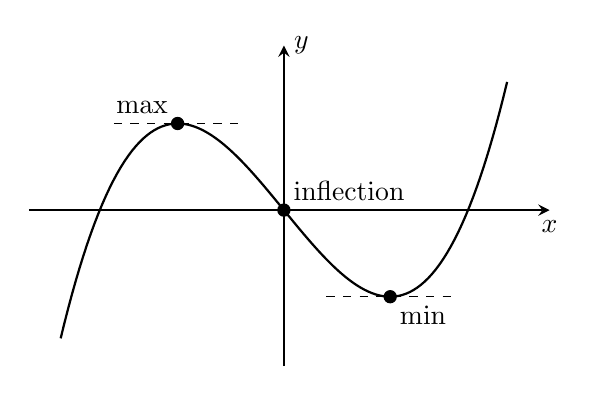
\begin{tikzpicture}[x=1.35cm,y=0.55cm,>=stealth]
  \draw[thick,->] (-2.4,0) -- (2.5,0) node[below] {$x$};
  \draw[thick,->] (0,-3.6) -- (0,3.8) node[right] {$y$};
  \draw[thick,domain=-2.1:2.1,samples=120,variable=\x] plot ({\x},{\x*\x*\x-3*\x});
  \draw[fill] (-1,2) circle (2.2pt) node[above left] {max};
  \draw[fill] (1,-2) circle (2.2pt) node[below right] {min};
  \draw[fill] (0,0) circle (2.2pt) node[above right] {inflection};
  \draw[dashed] (-1.6,2) -- (-0.4,2);
  \draw[dashed] (0.4,-2) -- (1.6,-2);
\end{tikzpicture}
\end{center}

ছবিটি $f(x) = x^{3} - 3x$-এর। এখানে $f' = 3x^{2}-3 = 3(x-1)(x+1)$, তাই critical
point $x = \pm 1$। আর $f'' = 6x$, তাই $f''(-1) = -6 < 0$ (সর্বোচ্চ) এবং
$f''(1) = 6 > 0$ (সর্বনিম্ন)। $f'' $ চিহ্ন বদলায় $x = 0$-এ, তাই সেটি
inflection point।

একটি সতর্কতা: এগুলো \emph{স্থানীয়} চরম মান। বন্ধ ব্যবধি $[a,b]$-তে সর্বোচ্চ ও
সর্বনিম্ন খুঁজতে হলে critical point-গুলোর মান আর দুই প্রান্তবিন্দুর মান সব
একসঙ্গে তুলনা করতে হয়; উপরের ছবিতেই দেখা যাচ্ছে যে ফাংশনটি $x$ বড় হলে
$2$ ছাড়িয়ে অনেক উপরে উঠে যায়।

\begin{example}
নির্দিষ্ট আয়তন $V$-এর একটি বদ্ধ নলাকার কৌটার পৃষ্ঠতল সর্বনিম্ন করতে হলে উচ্চতা
ও ব্যাসার্ধের সম্পর্ক কী হবে?
\end{example}

\begin{solbox}
৯ নম্বর অধ্যায়ে এই সমস্যাটি AM--GM দিয়ে সমাধান করা হয়েছিল; এবার
derivative দিয়ে করি এবং উত্তর মেলে কি না দেখি।

$V = \pi r^{2}h$ থেকে $h = \dfrac{V}{\pi r^{2}}$, তাই
\[
  S(r) = 2\pi r^{2} + 2\pi r h = 2\pi r^{2} + \frac{2V}{r} .
\]
Derivative নিই ($r > 0$):
\[
  S'(r) = 4\pi r - \frac{2V}{r^{2}} .
\]
$S'(r) = 0$ বসিয়ে $4\pi r^{3} = 2V$, অর্থাৎ $r^{3} = \dfrac{V}{2\pi}$, অর্থাৎ
$V = 2\pi r^{3}$। তখন
\[
  h = \frac{V}{\pi r^{2}} = \frac{2\pi r^{3}}{\pi r^{2}} = 2r .
\]

সত্যিই সর্বনিম্ন কি না যাচাই করি:
\[
  S''(r) = 4\pi + \frac{4V}{r^{3}} > 0
\]
সব $r>0$-এর জন্য, তাই এটি নিশ্চিতভাবে সর্বনিম্ন।

৯ নম্বর অধ্যায়ের উত্তরও ছিল $h = 2r$। দুটি সম্পূর্ণ আলাদা পদ্ধতি একই উত্তর
দিল, যা দুটোকেই বিশ্বাসযোগ্য করে। পার্থক্য একটাই: AM--GM-এ সঠিক ভাগ খুঁজে বের
করার বুদ্ধি লাগত, এখানে কেবল derivative নিয়ে শূন্য বসাতে হলো।
\end{solbox}

\prob{2} $f(x) = 2x^{3} - 3x^{2} - 12x + 5$-এর critical point নির্ণয় করো এবং
second derivative test দিয়ে প্রতিটিকে শ্রেণীবদ্ধ করো।

\begin{sol}
$f'(x) = 6x^{2} - 6x - 12 = 6(x-2)(x+1)$, তাই critical point $x = -1$ ও
$x = 2$।

$f''(x) = 12x - 6$। সুতরাং $f''(-1) = -18 < 0$, অর্থাৎ $x=-1$-এ স্থানীয়
সর্বোচ্চ, মান $f(-1) = -2-3+12+5 = 12$। আর $f''(2) = 18 > 0$, অর্থাৎ $x=2$-এ
স্থানীয় সর্বনিম্ন, মান $f(2) = 16-12-24+5 = -15$।
\end{sol}

\prob{2} $[0,3]$ ব্যবধিতে $f(x) = x^{3} - 3x$-এর সর্বোচ্চ ও সর্বনিম্ন মান
নির্ণয় করো।

\begin{sol}
$f'(x) = 3x^{2}-3 = 0$ দেয় $x = \pm 1$, কিন্তু $x=-1$ ব্যবধির বাইরে; তাই
বিবেচ্য বিন্দু $x = 1$ এবং দুই প্রান্ত $x = 0$, $x = 3$।
\[
  f(0) = 0, \qquad f(1) = -2, \qquad f(3) = 27 - 9 = 18 .
\]
সর্বনিম্ন $-2$ ($x=1$-এ), সর্বোচ্চ $18$ ($x=3$-এ)।

লক্ষ করো, সর্বোচ্চটি এসেছে প্রান্তবিন্দু থেকে, কোনো critical point থেকে নয়।
প্রান্ত পরীক্ষা করতে ভুলে গেলে উত্তর ভুল হতো।
\end{sol}

\prob{3} $f(x) = x^{4} - 4x^{3}$-এর জন্য বৃদ্ধি ও হ্রাসের ব্যবধি, concavity-র
ব্যবধি এবং inflection point নির্ণয় করো। $x = 0$ critical point হয়েও কেন চরম
মান নয়, ব্যাখ্যা করো।

\begin{sol}
$f'(x) = 4x^{3} - 12x^{2} = 4x^{2}(x-3)$।

$4x^{2} \geq 0$ সবসময়, তাই $f'$-এর চিহ্ন নির্ভর করে $(x-3)$-এর উপর:
$x < 3$-এ $f' < 0$ (হ্রাসমান, কেবল $x=0$-এ শূন্য) এবং $x > 3$-এ $f' > 0$
(বর্ধমান)। সুতরাং $x = 3$-এ স্থানীয় সর্বনিম্ন, মান $81 - 108 = -27$।

$x = 0$-ও critical point ($f'(0)=0$), কিন্তু তার দুই পাশেই $f' < 0$; চিহ্ন
বদলায়নি, তাই সেখানে চরম মান নেই। ফাংশনটি কেবল এক মুহূর্তের জন্য সমতল হয়ে
আবার নামতে থাকে।

$f''(x) = 12x^{2} - 24x = 12x(x-2)$। সুতরাং $f'' > 0$ যখন $x<0$ বা $x>2$
(concave upward), আর $f'' < 0$ যখন $0<x<2$ (concave downward)। দুই জায়গায়
চিহ্ন বদলায়, তাই inflection point $x = 0$ ও $x = 2$।

খেয়াল করো, second derivative test এখানে $x=0$-এ কিছু বলত না, কারণ
$f''(0) = 0$; first derivative test-ই উত্তর দিল।
\end{sol}

\prob{3} $a$ বাহুর একটি বর্গাকার টিনের পাত থেকে চার কোণে $x$ বাহুর বর্গ কেটে
বাদ দিয়ে বাকিটা ভাঁজ করে ঢাকনাবিহীন একটি বাক্স বানানো হলো। আয়তন সর্বাধিক
করতে $x$ কত নিতে হবে, এবং সেই সর্বাধিক আয়তন কত?

\begin{sol}
ভাঁজ করার পর ভূমি $(a-2x) \times (a-2x)$ এবং উচ্চতা $x$, তাই
\[
  V(x) = x(a-2x)^{2}, \qquad 0 < x < \frac{a}{2} .
\]
Product rule ও chain rule প্রয়োগ করে
\[
  V'(x) = (a-2x)^{2} + x \cdot 2(a-2x)(-2)
        = (a-2x)\bigl[ (a-2x) - 4x \bigr]
        = (a-2x)(a-6x) .
\]
$0 < x < a/2$-এ $a-2x > 0$, তাই $V' = 0$ দেয় $x = \dfrac{a}{6}$। বাঁয়ে
$V' > 0$ ও ডানে $V' < 0$, তাই এটি সর্বাধিক।
\[
  V\left( \frac{a}{6} \right)
  = \frac{a}{6}\left( a - \frac{a}{3} \right)^{2}
  = \frac{a}{6} \cdot \frac{4a^{2}}{9} = \frac{2a^{3}}{27} .
\]
অর্থাৎ মূল পাতের ঘনফলের তুলনায় নয়, বরং $a^{3}$-এর প্রায় $7.4$ শতাংশ।
\end{sol}

\prob{4} আলো এক মাধ্যম থেকে আরেক মাধ্যমে যায় এবং দুই মাধ্যমে তার দ্রুতি
যথাক্রমে $v_{1}$ ও $v_{2}$। বিভেদতল থেকে $a$ দূরত্বে $A$ বিন্দু এবং অন্য পাশে
$b$ দূরত্বে $B$ বিন্দু; তাদের পাদবিন্দু দুটির মধ্যে অনুভূমিক দূরত্ব $d$। আলো
বিভেদতলের যে বিন্দুতে আঘাত করে সেটি $A$-এর পাদবিন্দু থেকে $x$ দূরে।
\begin{enumerate}
  \item মোট সময় $T(x)$-এর রাশি লেখো।
  \item $T$ সর্বনিম্ন হওয়ার শর্ত থেকে দেখাও যে
        $\dfrac{\sin\theta_{1}}{v_{1}} = \dfrac{\sin\theta_{2}}{v_{2}}$,
        যেখানে $\theta_{1}, \theta_{2}$ হলো বিভেদতলের অভিলম্বের সঙ্গে কোণ।
\end{enumerate}

\begin{sol}
\begin{enumerate}
  \item প্রথম মাধ্যমে পথের দৈর্ঘ্য $\sqrt{a^{2}+x^{2}}$ এবং দ্বিতীয়টিতে
        $\sqrt{b^{2}+(d-x)^{2}}$। সুতরাং
        \[
          T(x) = \frac{\sqrt{a^{2}+x^{2}}}{v_{1}}
               + \frac{\sqrt{b^{2}+(d-x)^{2}}}{v_{2}} .
        \]
  \item Chain rule প্রয়োগ করে
        \[
          T'(x) = \frac{x}{v_{1}\sqrt{a^{2}+x^{2}}}
                - \frac{d-x}{v_{2}\sqrt{b^{2}+(d-x)^{2}}} .
        \]
        এখন জ্যামিতি দেখি: $\theta_{1}$ হলো আপতিত রশ্মি ও অভিলম্বের কোণ, আর
        সমকোণী ত্রিভুজ থেকে
        \[
          \sin\theta_{1} = \frac{x}{\sqrt{a^{2}+x^{2}}}, \qquad
          \sin\theta_{2} = \frac{d-x}{\sqrt{b^{2}+(d-x)^{2}}} .
        \]
        সুতরাং $T'(x) = \dfrac{\sin\theta_{1}}{v_{1}} -
        \dfrac{\sin\theta_{2}}{v_{2}}$, এবং $T'(x) = 0$ দেয়
        \[
          \frac{\sin\theta_{1}}{v_{1}} = \frac{\sin\theta_{2}}{v_{2}} .
        \]
        এটিই Snell-এর সূত্র। এটি যে সর্বনিম্ন (সর্বোচ্চ নয়) তা দেখা যায়
        $T'$-এর চিহ্ন থেকে: $x$ বাড়লে প্রথম পদ বাড়ে ও দ্বিতীয় পদ কমে, তাই
        $T'$ কড়াভাবে বর্ধমান এবং শূন্য অতিক্রম করে ঋণাত্মক থেকে ধনাত্মকে।
\end{enumerate}
আলো যে ``সবচেয়ে কম সময়ের পথ'' নেয়, এই নীতিটি Fermat-এর নামে পরিচিত; উপরের
হিসাবটি দেখাচ্ছে যে প্রতিসরণের সূত্র তার সরাসরি ফল।
\end{sol}

\section{আংশিক ডেরিভেটিভ}

এতক্ষণ প্রতিটি ফাংশনের একটিমাত্র ইনপুট ছিল। বাস্তবে তা বিরল। একটি ধাতব পাতের
তাপমাত্রা নির্ভর করে দুটি স্থানাঙ্কের উপর; গ্যাসের চাপ নির্ভর করে আয়তন ও
তাপমাত্রার উপর।

\begin{idea}[দুই চলকের ফাংশন]
$f$ যদি সমতলের কোনো অঞ্চল $D$-এর প্রতিটি বিন্দু $(x,y)$-কে একটি বাস্তব সংখ্যা
$f(x,y)$-এর সঙ্গে যুক্ত করে, তবে $f$ হলো দুই চলকের ফাংশন। $D$ তার domain, আর
তার লেখচিত্র হলো ত্রিমাত্রিক স্থানে $z = f(x,y)$ সমীকরণের তল (surface)।
\end{idea}

উদাহরণ: $f(x,y) = x^{2}+y^{2}$-এর domain গোটা সমতল, আর তার তল একটি বাটির মতো
আকৃতি; $z$ ধ্রুবক রেখে কাটলে বৃত্ত পাওয়া যায় (১২ নম্বর অধ্যায়ের
$x^{2}+y^{2} = c$)।

তল নিয়ে কীভাবে derivative নেব? সমস্যা হলো, তলের একটি বিন্দু থেকে অসংখ্য দিকে নড়া (অর্থাৎ স্বাধীন চলকের মান পরিবর্তন করা)
যায়, প্রতিটি দিকে ঢাল আলাদা। সবচেয়ে সহজ সমাধান: একবারে একটি দিক।

\begin{idea}[আংশিক derivative]
\[
  \frac{\partial f}{\partial x}(x,y)
  = \lim_{h \to 0} \frac{f(x+h,\, y) - f(x,\, y)}{h} ,
\]
অর্থাৎ $y$-কে ধ্রুবক ধরে কেবল $x$-এর সাপেক্ষে সাধারণ derivative। একইভাবে
$\dfrac{\partial f}{\partial y}$-তে $x$ ধ্রুবক। এদের $f_{x}$ ও $f_{y}$-ও লেখা হয়।
\end{idea}

\begin{center}
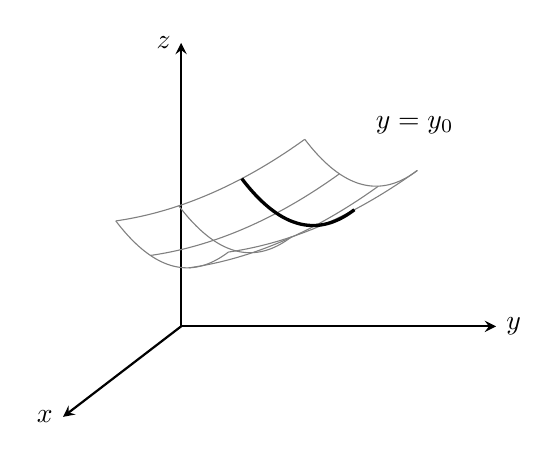
\begin{tikzpicture}[scale=1.0,>=stealth]
  \draw[thick,->] (0,0) -- (-1.5,-1.15) node[left] {$x$};
  \draw[thick,->] (0,0) -- (4.0,0) node[right] {$y$};
  \draw[thick,->] (0,0) -- (0,3.6) node[left] {$z$};
  \foreach \yy in {0.6,1.4,2.2,3.0}{
    \draw[gray,thin,domain=0:2.6,samples=40,variable=\x]
      plot ({-0.55*\x+\yy},{-0.42*\x+0.9+0.22*\x*\x+0.12*\yy*\yy});
  }
  \foreach \xx in {0,0.9,1.8,2.6}{
    \draw[gray,thin,domain=0.6:3.0,samples=40,variable=\y]
      plot ({-0.55*\xx+\y},{-0.42*\xx+0.9+0.22*\xx*\xx+0.12*\y*\y});
  }
  \draw[very thick,domain=0:2.6,samples=60,variable=\x]
      plot ({-0.55*\x+2.2},{-0.42*\x+0.9+0.22*\x*\x+0.12*2.2*2.2});
  \node[right] at (2.35,2.55) {$y=y_{0}$};
\end{tikzpicture}
\end{center}

ছবিটি জ্যামিতিক অর্থ দেখাচ্ছে। $y = y_{0}$ ধ্রুবক রাখা মানে তলটিকে একটি উল্লম্ব
সমতল দিয়ে কাটা; কাটা দাগে যে বক্ররেখা পাওয়া যায় (মোটা রেখাটি) সেটি এক চলকের
সাধারণ ফাংশন, আর $\dfrac{\partial f}{\partial x}$ হলো ঠিক ওই বক্ররেখার ঢাল।

চিহ্নটি খেয়াল করো: $\partial$, সাধারণ $d$ নয়। পার্থক্যটা নিছক সাজসজ্জা নয়;
$\partial$ মানে ``বাকি চলকগুলোর পরিবর্তন  আটকে রাখা হয়েছে''।

\begin{example}
$f(x,y) = x^{2}y + \sin y$ হলে $f_{x}$, $f_{y}$ এবং দ্বিতীয় স্তরের চারটি
আংশিক derivative নির্ণয় করো।
\end{example}

\begin{solbox}
$f_{x}$ বের করতে $y$-কে ধ্রুবক ভাবি; তখন $\sin y$ একটি ধ্রুবক, যার derivative
শূন্য:
\[
  f_{x} = 2xy .
\]
$f_{y}$ বের করতে $x$ ধ্রুবক; তখন $x^{2}$ একটি ধ্রুবক গুণক:
\[
  f_{y} = x^{2} + \cos y .
\]
দ্বিতীয় স্তর:
\[
  f_{xx} = 2y, \qquad f_{yy} = -\sin y, \qquad
  f_{xy} = \frac{\partial}{\partial y}(2xy) = 2x, \qquad
  f_{yx} = \frac{\partial}{\partial x}\left( x^{2}+\cos y \right) = 2x .
\]
শেষ দুটি সমান। এটি কাকতালীয় নয়: যেসব ফাংশনের দ্বিতীয় আংশিক derivative
continuous, তাদের জন্য $f_{xy} = f_{yx}$ সবসময়। এই ফলটি এখানে প্রমাণ করা হচ্ছে
না, ধরে নেওয়া হচ্ছে।
\end{solbox}

\begin{idea}[একাধিক চলকের chain rule]
$x$ ও $y$ দুটিই যদি $t$-এর উপর নির্ভর করে, তবে
\[
  \frac{df}{dt} = \frac{\partial f}{\partial x}\frac{dx}{dt}
                + \frac{\partial f}{\partial y}\frac{dy}{dt} .
\]
\end{idea}

এটিও এখানে প্রমাণ করা হচ্ছে না। এখানে
$\dfrac{df}{dt}$-কে বলে total derivative আর $\dfrac{\partial f}{\partial x}$-কে
partial derivative।

\begin{remark}
আংশিক derivative পদার্থবিজ্ঞানে সর্বত্র। তাপগতিবিদ্যায় প্রায় প্রতিটি রাশিই
কয়েকটি চলকের ফাংশন, তাই সেখানে $\partial$ ছাড়া একটি লাইনও লেখা যায় না।
তরঙ্গ সমীকরণ, তাপ সমীকরণ, Maxwell-এর সমীকরণ, সবই আংশিক derivative-এ লেখা।
২১ নম্বর অধ্যায়ে এদের একটি সুসংহত রূপ আসবে: তিনটি আংশিক derivative একসঙ্গে
নিয়ে গঠিত ভেক্টর, যার নাম gradient।
\end{remark}

\prob{2} $f(x,y) = x^{3}y^{2} - 4xy + y$ হলে $f_{x}$, $f_{y}$, $f_{xx}$,
$f_{xy}$ ও $f_{yx}$ নির্ণয় করো এবং শেষ দুটি সমান কি না যাচাই করো।

\begin{sol}
$y$ ধ্রুবক ধরে: $f_{x} = 3x^{2}y^{2} - 4y$।

$x$ ধ্রুবক ধরে: $f_{y} = 2x^{3}y - 4x + 1$।

$f_{xx} = \dfrac{\partial}{\partial x}\left( 3x^{2}y^{2}-4y \right) = 6xy^{2}$।

$f_{xy} = \dfrac{\partial}{\partial y}\left( 3x^{2}y^{2}-4y \right)
= 6x^{2}y - 4$।

$f_{yx} = \dfrac{\partial}{\partial x}\left( 2x^{3}y - 4x + 1 \right)
= 6x^{2}y - 4$।

শেষ দুটি সমান, যেমনটা প্রত্যাশিত।
\end{sol}

\prob{4} আদর্শ গ্যাসের সমীকরণ $PV = nRT$, যেখানে $n$ ও $R$ ধ্রুবক।
\begin{enumerate}
  \item $P$-কে $V$ ও $T$-এর ফাংশন ধরে $\dfrac{\partial P}{\partial V}$ ও
        $\dfrac{\partial P}{\partial T}$ নির্ণয় করো।
  \item $V$ ও $T$ দুটিই সময়ের সঙ্গে বদলালে $\dfrac{dP}{dt}$ লেখো।
  \item প্রমাণ করো যে
        $\dfrac{\partial P}{\partial V} \cdot
         \dfrac{\partial V}{\partial T} \cdot
         \dfrac{\partial T}{\partial P} = -1$।
\end{enumerate}

\begin{sol}
\begin{enumerate}
  \item $P = \dfrac{nRT}{V}$, তাই
        \[
          \frac{\partial P}{\partial V} = -\frac{nRT}{V^{2}}, \qquad
          \frac{\partial P}{\partial T} = \frac{nR}{V} .
        \]
  \item একাধিক চলকের chain rule প্রয়োগ করে
        \[
          \frac{dP}{dt} = \frac{nR}{V}\frac{dT}{dt}
                        - \frac{nRT}{V^{2}}\frac{dV}{dt} .
        \]
  \item এবার অন্য দুটি চলককে আলাদা করে লিখি:
        $V = \dfrac{nRT}{P}$ দেয় $\dfrac{\partial V}{\partial T} =
        \dfrac{nR}{P}$, আর $T = \dfrac{PV}{nR}$ দেয়
        $\dfrac{\partial T}{\partial P} = \dfrac{V}{nR}$। গুণ করি:
        \[
          \left( -\frac{nRT}{V^{2}} \right)
          \left( \frac{nR}{P} \right)
          \left( \frac{V}{nR} \right)
          = -\frac{nRT}{VP} = -1 ,
        \]
        কারণ $PV = nRT$।
\end{enumerate}
তৃতীয় অংশটি মনে রাখার মতো। $\partial$-গুলোকে ভগ্নাংশ ভেবে কাটাকাটি করলে
উত্তর $+1$ আসত, অথচ সঠিক উত্তর $-1$। আংশিক derivative ভগ্নাংশ নয়, আর এই
উদাহরণটাই তার সবচেয়ে পরিষ্কার প্রমাণ।
\end{sol}

\section{টেইলর সিরিজ}

শেষ অনুচ্ছেদটি ছোট, এবং উদ্দেশ্যও সীমিত: একটি ধারণা আর কয়েকটি সম্প্রসারণ
হাতে ধরিয়ে দেওয়া, যেগুলো পদার্থবিজ্ঞানে বারবার লাগে।

মূল প্রশ্নটা এই: $\sin x$ বা $e^{x}$ ধরনের ফাংশনের মান হাতে হিসাব করা কঠিন,
কিন্তু polynomial-এর মান বের করা সহজ। তাহলে কি একটি ফাংশনকে polynomial দিয়ে
বদলে ফেলা যায়?

\begin{idea}[Taylor সহগ]
$x = 0$-এর কাছে $f$-কে
\[
  f(x) \approx c_{0} + c_{1}x + c_{2}x^{2} + \cdots + c_{n}x^{n}
\]
আকারে লিখতে চাইলে, এবং দুই পাশের মান ও প্রথম $n$টি derivative
$x=0$-তে মিলাতে চাইলে,
\[
  c_{k} = \frac{f^{(k)}(0)}{k!} .
\]
\end{idea}

কারণটা পরিষ্কার। আর তা নিজে নিজে বের করার চেষ্টা করো (না পারলে \hyperlink{https://www.youtube.com/watch?v=3d6DsjIBzJ4}{এই ভিডিওটা} দেখতে পারো)। $x = a$-এর চারপাশে এই কাজটা করতে চাইলে $x$-এর জায়গায় $(x-a)$ বসাও; $a=0$ ক্ষেত্রটিকে
বলে Maclaurin series।

উদাহরণ হিসেবে $f(x) = e^{x}$ নাও। প্রতিটি derivative আবার $e^{x}$, তাই
$f^{(k)}(0) = 1$ সব $k$-এর জন্য, এবং $c_{k} = \dfrac{1}{k!}$।

\begin{idea}[কয়েকটি দরকারি সম্প্রসারণ]
\[
  e^{x} = 1 + x + \frac{x^{2}}{2!} + \frac{x^{3}}{3!} + \cdots
\]
\[
  \sin x = x - \frac{x^{3}}{3!} + \frac{x^{5}}{5!} - \cdots, \qquad
  \cos x = 1 - \frac{x^{2}}{2!} + \frac{x^{4}}{4!} - \cdots
\]
\[
  \ln(1+x) = x - \frac{x^{2}}{2} + \frac{x^{3}}{3} - \cdots
  \qquad (|x| < 1)
\]
\[
  (1+x)^{n} = 1 + nx + \frac{n(n-1)}{2!}x^{2} + \cdots
\]
\end{idea}

\begin{remark}
এখানে যা \emph{করা হয়নি} সেটা স্পষ্ট করে বলা দরকার। উপরের সমান চিহ্নগুলো
আসলে একটি অতিরিক্ত দাবি করছে: অসীম ধারাটি সত্যিই ফাংশনটির সমান, এবং কোন
কোন $x$-এর জন্য সমান। ধারার অভিসৃতি (convergence) নিয়ে এই সিরিজে কোনো
অধ্যায় নেই, তাই এই দাবিটি এখানে প্রমাণ করা হচ্ছে না, ধরে নেওয়া হচ্ছে।
নিরাপদ পড়াটা হলো: এগুলো ছোট $|x|$-এর জন্য আসন্নীকরণ, আর যত বেশি পদ নেবে তত
ভালো। $\ln(1+x)$-এর ক্ষেত্রে $|x|<1$ শর্তটি আলাদা করে লেখা হয়েছে, কারণ
সেখানে সীমাবদ্ধতাটি প্রকট।

অলিম্পিয়াডের হিসাবের জন্য পুরো ধারাটা প্রায় কখনোই লাগে না; লাগে প্রথম দুই বা
তিনটি পদ। সেটুকুই এই অনুচ্ছেদের আসল সম্পদ।
\end{remark}

\begin{center}
\begin{tikzpicture}[x=0.85cm,y=0.85cm,>=stealth]
  \draw[thick,->] (-4.3,0) -- (4.5,0) node[below] {$x$};
  \draw[thick,->] (0,-2.4) -- (0,2.5) node[left] {$y$};
  \begin{scope}
   \clip (-4.3,-2.3) rectangle (4.3,2.3);
   \draw[very thick,domain=-4.2:4.2,samples=150,variable=\x] plot ({\x},{sin(\x r)});
   \draw[dashed,domain=-4.2:4.2,samples=60,variable=\x] plot ({\x},{\x});
   \draw[dash pattern=on 4pt off 2pt,domain=-4.2:4.2,samples=120,variable=\x]
        plot ({\x},{\x-(\x*\x*\x)/6});
  \end{scope}
  \node[right] at (2.4,1.25) {$y=\sin x$};
  \node[right] at (1.3,2.1) {$y=x$};
  \node[below right] at (2.9,-1.25) {$y=x-\tfrac{x^{3}}{6}$};
\end{tikzpicture}
\end{center}

ছবিটি একটি কথা পরিষ্কার করে দেয়। মূলবিন্দুর কাছে $y=x$ রেখাটি $\sin x$-এর
সঙ্গে মিশে আছে, কিন্তু দূরে গিয়ে ছাড়াছাড়ি হয়ে যায়; দ্বিতীয় আসন্নীকরণটি
আরও দূর পর্যন্ত লেগে থাকে। এটিই ১৩ নম্বর অধ্যায়ের ছোট কোণের সূত্র, এবার
তার উৎসসহ: $\sin\theta \approx \theta$ হলো ধারার প্রথম পদ, আর
$\cos\theta \approx 1 - \dfrac{\theta^{2}}{2}$ হলো প্রথম দুটি পদ। ওখানে
পাওয়া ভুলের সীমা $\theta^{3}/2$-এর সঙ্গে মিলিয়ে দেখো: ধারার প্রথম বাদ পড়া
পদটি ঠিক $\theta^{3}/6$।

\begin{remark}
$(1+x)^{n} \approx 1 + nx$ আসন্নীকরণটি পদার্থবিজ্ঞানে ছোট কোণের সূত্রের পরেই
সবচেয়ে বেশি ব্যবহৃত। যেমন আপেক্ষিকতায়
\[
  \gamma = \frac{1}{\sqrt{1 - v^{2}/c^{2}}}
  = \left( 1 - \frac{v^{2}}{c^{2}} \right)^{-1/2}
  \approx 1 + \frac{v^{2}}{2c^{2}} ,
\]
আর সেখান থেকেই গতিশক্তির চেনা রূপ $\tfrac{1}{2}mv^{2}$ বেরিয়ে আসে। মনে রেখো,
$n$ এখানে পূর্ণসংখ্যা হতে হবে না; ৮ নম্বর অধ্যায়ের binomial theorem-এর
এটিই সাধারণ রূপ।
\end{remark}

\prob{3} Maclaurin সহগের সূত্র ব্যবহার করে $\cos x$-এর প্রথম তিনটি অশূন্য পদ
বের করো। এরপর $\cos(0.2)$-এর মান দুই পদ ও তিন পদ দিয়ে হিসাব করে প্রকৃত মান
$0.980067$-এর সঙ্গে তুলনা করো।

\begin{sol}
$f(x) = \cos x$-এর derivative-গুলো ঘুরেফিরে আসে:
$f' = -\sin x$, $f'' = -\cos x$, $f''' = \sin x$, $f^{(4)} = \cos x$।
$x=0$-এ মানগুলো যথাক্রমে $1, 0, -1, 0, 1$। সুতরাং
\[
  c_{0} = 1, \quad c_{1} = 0, \quad c_{2} = -\frac{1}{2!}, \quad
  c_{3} = 0, \quad c_{4} = \frac{1}{4!} ,
\]
অর্থাৎ
\[
  \cos x \approx 1 - \frac{x^{2}}{2} + \frac{x^{4}}{24} .
\]

এখন $x = 0.2$:

দুই পদে: $1 - \dfrac{0.04}{2} = 0.98$; ভুল $0.000067$।

তিন পদে: $0.98 + \dfrac{0.0016}{24} = 0.98 + 0.0000667 = 0.9800667$; ভুল
প্রায় $3 \times 10^{-8}$।

একটি বাড়তি পদ ভুলকে প্রায় দুই হাজার গুণ কমিয়ে দিল। ছোট $x$-এর জন্য ধারাটি
এত দ্রুত ভালো হয় বলেই এটি এত কাজের।
\end{sol}

\end{document}